

\section{Installation Guide}
\label{sec:Install}

In this section, we provide instructions on how to integrate our developed \ac{sihft} passes within the LLVM codebase.
This allows us later to carry out various \ac{sihft} transformations during LLVM backend compilation in generating
RISCV code.

\subsection{Development System}
The instructions given in this user manual are expected to work on any Linux machine. Specifically, we have prepared
this manual while developing on a freshly installed Ubuntu 20.04 PC.

\subsubsection{Ubuntu Packages}
Following packages are needed to be installed:

\begin{itemize}
 \item{C++ compiler like gcc/g++}
 \item{CMake}
 \item{git}
\end{itemize}

Following commands can be used to install them:

\begin{lstlisting}[language=bash, frame=single, basicstyle=\small\ttfamily]
$ sudo apt update
$ sudo apt install build-essential cmake git
  \end{lstlisting}

\subsection{Build LLVM Project}
\label{sec:build-llvm}
The LLVM Project has to be compiled from source. We recommend downloading version 13.0.0 from LLVM Releases webpage:
\\\\
\url{https://releases.llvm.org/} \\

With the downloaded source package extracted, execute the following commands on your bash shell to build
llvm project from source:

\begin{framed}
 \begin{lstlisting}[language=bash, basicstyle=\small\ttfamily]
$ cd <llvm_src_folder>
$ mkdir build
$ cd build
$ cmake -DCMAKE_BUILD_TYPE=Release
        -DCMAKE_INSTALL_PREFIX=<install_location>
        -DCMAKE_CXX_STANDARD=17
        -DLLVM_ENABLE_PROJECTS=clang
        -DLLVM_TARGETS_TO_BUILD=RISCV
        -DLLVM_ENABLE_ASSERTIONS=ON
        ../llvm
$ make
  \end{lstlisting}
\end{framed}

\textit{NOTE: The paths mentioned above as $<$...$>$ need to be adapted as per your filesystem.} \\

In the \texttt{<build>/bin} directory, we should now see llvm executable programs and utilities like
\texttt{clang}, \texttt{llc} etc. Run them to make sure they are built fine. For example, we can run the
static compiler \texttt{llc} to make sure that RISCV targets are supported as shown in Fig.~\ref{fig:llc}. \\

\begin{figure}[htb]
 \centering
 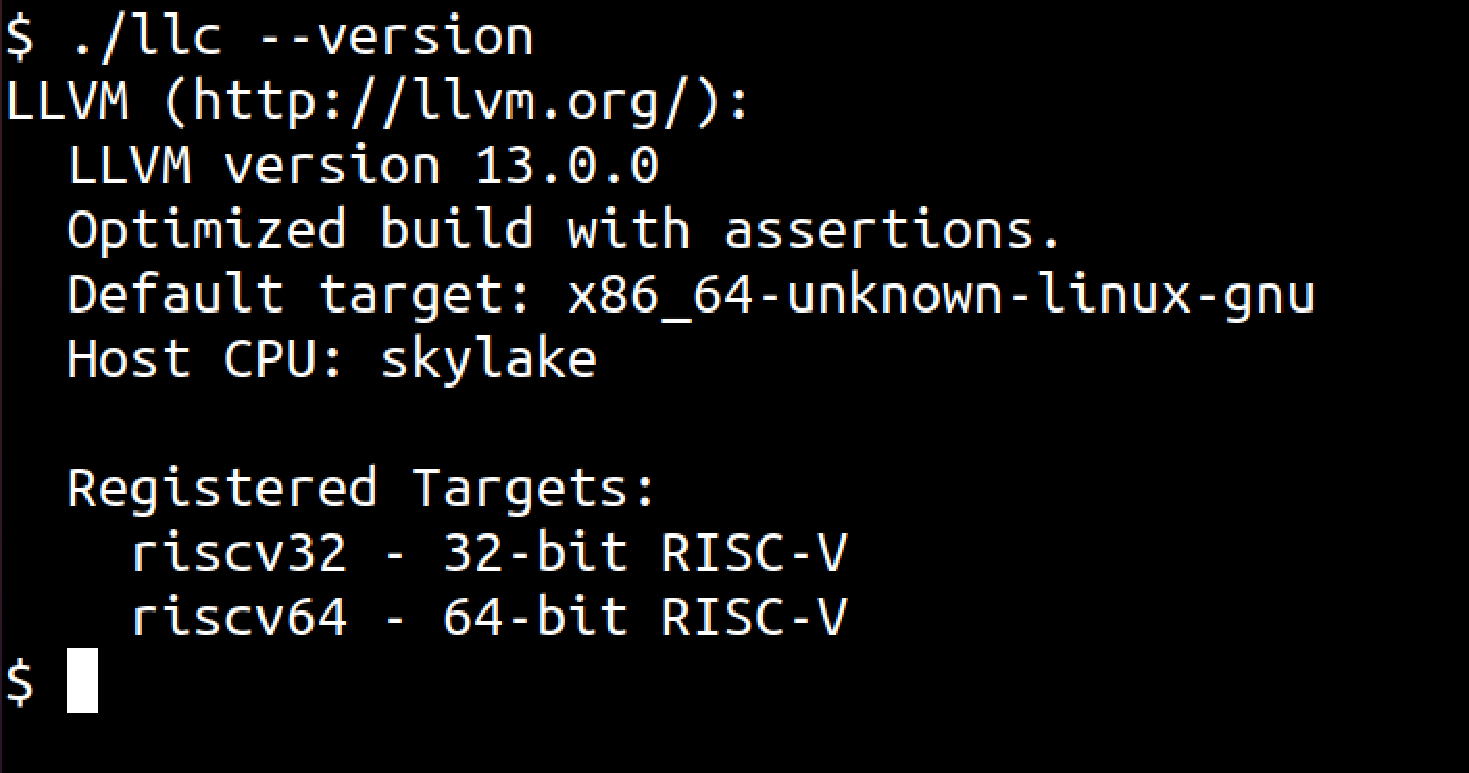
\includegraphics[width=0.8\linewidth]{figs/llc.pdf}
 \caption{Expected output of sanely built \texttt{llc}}
 \label{fig:llc}
\end{figure}

\textit{NOTE: Make using parallel jobs (\texttt{make -jN}) would help significantly to reduce the compile time
 for a large codebase like LLVM. However, we encourage to do this on a server. For systems having lesser memory, make
 with parallel jobs has to be used cautiously, as the command could fail due to memory exhaustion issues.}

% \newpage
\subsection{Integrate \ac{sihft} Passes}
The first step is to clone our open-source \texttt{compas-ft-riscv} repository within the LLVM source tree. Afterwards,
the patch is applied on RISCV backend in order to register the new transformation passes. Finally, the LLVM project
is rebuilt.

The corresponding shell commands are shown below. Here \texttt{<path\_to\_patch>} variable should be substituted
with a compatible patch file. For this, we provide various patches in our passes repository.
Each patch is compatible with a specific llvm project source tree.
In case this tutorial is followed to build llvm project using Sec.~\ref{sec:build-llvm},
the corresponding patch is to be found at:\\\\
\texttt{compas-ft-riscv/patches/llvm13.0.0\_src.patch}

\begin{framed}
 \begin{lstlisting}[language=bash, basicstyle=\small\ttfamily]
$ cd <llvm_src_folder>/llvm/lib/Target/RISCV/
$ git clone https://github.com/tum-ei-eda/compas-ft-riscv
$ cd <llvm_src_folder>
$ patch -s -p0 < <path_to_patch>
$ cd build
$ make
$ make install
\end{lstlisting}
\end{framed}

Here, at the end we install the built llvm compiler infrastructure. Again make sure that the compiler is installed fine
by using Fig.~\ref{fig:llc}.
